\chapter{

\section{Oveview} 

\subsection{Actors}

The overview and flow of the Dapp developed is shown in \textbf{Figure 1}. 
The \textbf{Actors} involved in the system are:

\begin{outline}
    \1 \textbf{User}: It's the \textit{end user}. It use the web-app to send old clothes and purchase from Reclothes store
    \1 \textbf{Reclothes Admin}: It's the \textit{system admin}, it perform the actions in order to handle the system
    \1 \textbf{Producer}: It's part of the upcycling process. It receive the materials to perform the recycling process
\end{outline}

Each of that access to the system wich different permission and priviledges. Once the user is logged in, 
It could access to several features. It's possible to split the overview flow
into 2 subflow starting from Reclothes actor, the \textbf{User side} and the \textbf{Producer side}.

\begin{outline}[enumerate]
	\1 \textbf{User Side}
    \2 User send Box with old clothes and receive Fabric points and ERC20 Token
    \2 User purchase items inside dapp store using Fabric points and ERC20 Token
    \1 \textbf{Producer Side}
    \2 Reclothes send clothes box with old matherials and receive Regeneration Credits
    \2 Reclothes spend the Regeneration Credits to purchase upcycled clothes by Producer
\end{outline}

\subsection{Token echanged}

The \textbf{Token} exchanged over the networks will be:

\begin{outline}[enumerate]
	\1 \textbf{Over Fabric Net}
    \2 \textbf{User Token}: It's a point used to handle part of payment system, points based, related to clothes
    shipping from User to Reclothes and viceversa.
    \2 \textbf{Regeneration Credits}: It's a point used to handle part of credit system, points based, related to clothes
    shipping from Reclothes to Producers and viceversa.

    \1 \textbf{Over Ethereum Net}
    \2 \textbf{CO2 Token}: It's and ERC20 Token run over public network in charge to handle part of payments
    related to clothes shipping from User to Reclothes and viceversa.
\end{outline}


\begin{figure}[h!]
	\centering
	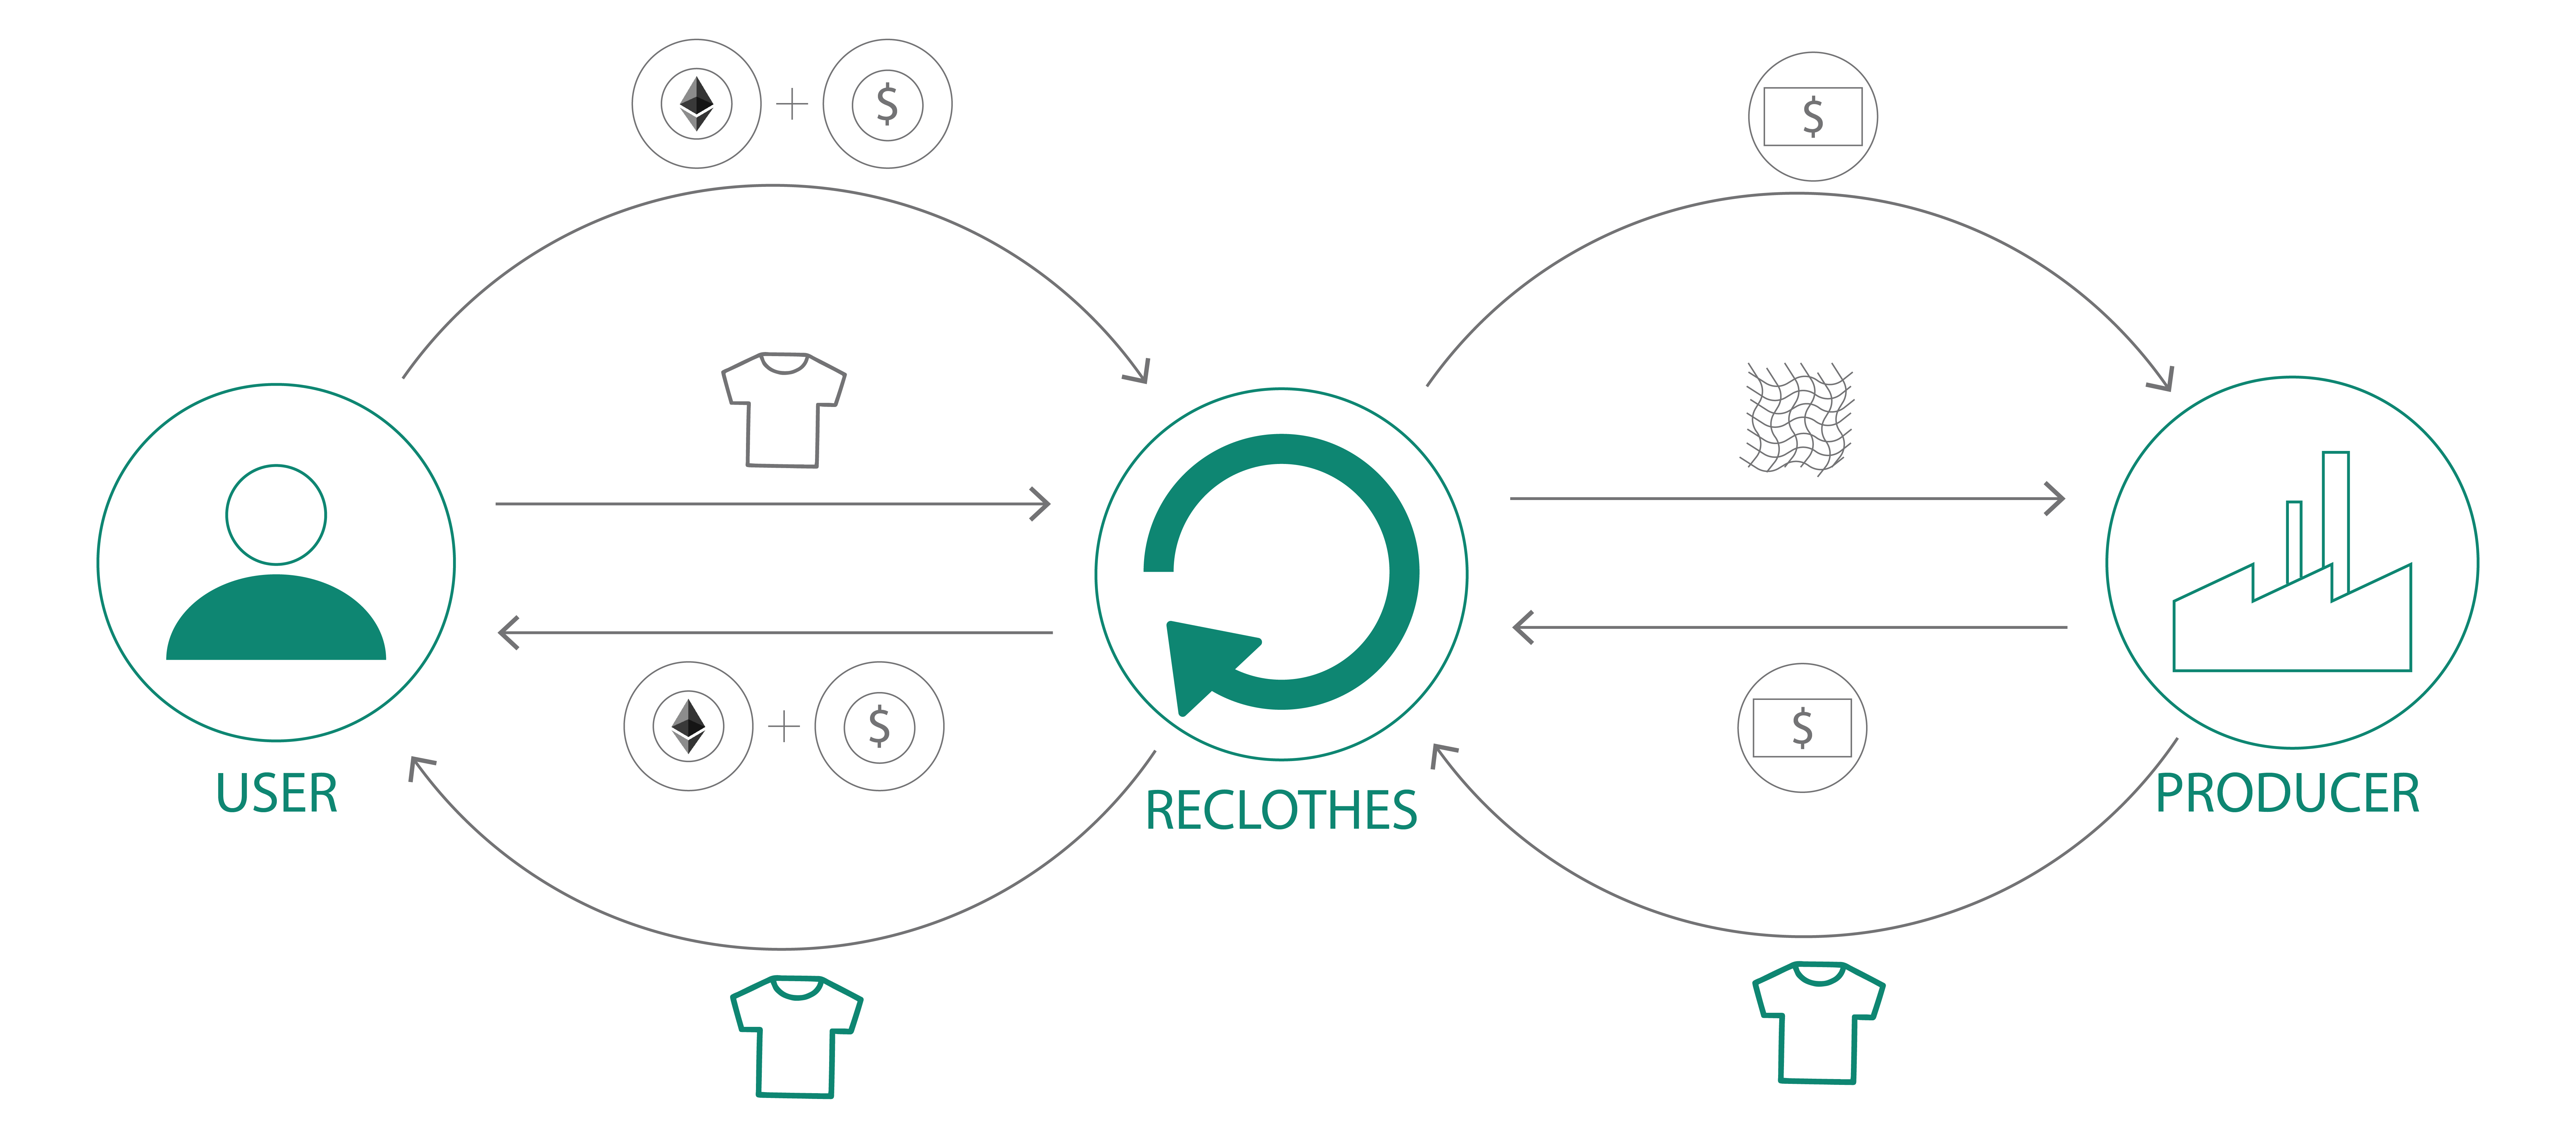
\includegraphics[totalheight=6cm]{img/use-case-schema.png}
	\caption{UseCase Overview}
	\label{fig:schema}
\end{figure}


\section{Technologies used to perform crosschain interaction}

\subsection{Tool Used}

\begin{outline}
    \1 \textbf{Metamask}: It's used as ethereum wallet to perform and sign the transactions started by dapp 
    \1 \textbf{Web3}: It's the software library used to interact with smart contract
    \1 \textbf{Fab3 Proxy}: It map the Web3 API with the Fabric SDK in order to interact with
    Fabric network. It perform a mapping between the Fabric Identity (X.509) with an eth address, generated on the fly,
    used to perform dapp call. 
    \1 \textbf{Fabric Chaincode EVM}: It's the EVM chaincode that allow to run Solidity smart contract
    over the Fabric network
    \1 \textbf{Expressjs}: Web Framework used to develop web-app and smart contract API 
    \1 \textbf{Infura}: allow to run a Ethereum node in order to set an endpoint used to interact with own contract.
    \1 \textbf{Docker}: The fabric network components run inside Docker containers.
\end{outline}

Figure ~\ref{architecturalFlow} show The Architectural Flow and how the technologies is used and interact each other.

\begin{figure}[h!]
	\centering
	\includegraphics[totalheight=13cm]{img/architectural_flow.png}
	\caption{Architectural Flow}
    \label{architecturalFlow}
\end{figure}
 
\section{Use Cases}

\subsection{UseCase 1 - User Side}

As shown in \textbf{Figure 2} both Actors User and Reclothes Admin, once is logged in, access to a set
of features. The Use case diagram show all the action that both users could perform over the networks and
tha flows that each actions follow. The features are split over the two network, the Fabric one and the 
Ethereum one. 

The Internal Flow of the \textit{\bf{Send Box}} macro process is the follow one:

\begin{outline}[enumerate]
    \1 User send box with old clothes
    \1 Reclothes Admin receive box, evaluate it
    \1 The web app perform the payments from Reclothes Account to User Account
    \1 Once both transactions succed, both token are accredited and User could spend it
\end{outline}

\subsubsection{Transactions}

The two process that start the transactions are the \textit{\bf{Evaluation}} performed by The Reclothes Admin
and the \textit{\bf{Purchase Items}} performed by the Users over the platform store. 

\\

\begin{outline}[enumerate]
    \1 The \textit{\bf{Evaluation}} process works in the following way:
    \2 Reclothes Admin visualize the next pending request to be evaluated
    \2 Reclothes Admin evaluate it and set an amount value of Fabric points and ERC20 Token to be send
    \3 The points are sent over Fabric network invoking a chaincode function
    \3 The ERC20 Token are send over Ethereum network (Ropsten), sending the token to the ETH Address stored
        in the smart contract during the User Registration Phase.
    \2 Once both transactions succed, both tokens are accredited and User could spend it

    \1 The \textit{\bf{Purchase Items}} process in a similar way:
    \2 User choose the items to purchase over the web-app store
    \2 Reclothes Admin evaluate it and set a value amount of Fabric points and ERC20 Token to send
    \3 The points are sent over Fabric network invoking a chaincode function
    \3 The ERC20 Token are send over Ethereum network (Ropsten), sending the token to the ETH Address stored
        in the smart contract during the User Registration Phase.
    \2 Once both transactions succed, both token are accredited and User could spend it
\end{outline}

\begin{figure}[h!]
	\centering
	\includegraphics[totalheight=15cm]{img/use_case1.png}
	\caption{UseCase 1}
	\label{fig:usecase1}
\end{figure}


\subsection{UseCase 2 - Producer Side}

The Use case diagram shown in \textbf{Figure 3} describe how Reclothes Admin and Producer interact each other.
In this case all the features are performed over the Hyperledger Fabric network.

\newline \\
We could split the flow into two subflow, the first one from Reclothes to Producer, that we could identify
with the two actions \textit{Send Box} and \textit{Purchase Box}, on the other hand the second subflow
from Producer to Reclothes is summarize into \textit{Evaluate Material} function. 

\newline \\
All the asset exchange is handle using \textbf{Regeneration Credits} a Fabric token exchanged
and handle by the Fabric chaincode and running over Fabric network.

\\
\begin{outline}[enumerate]
    \1 \textbf{from Reclothes to Producer}   
    \2 \textbf{Send Box}
    \3 Send Box with old materials to be recycled by the Producer Company
    \3 Receive \textbf{Regeneration Credits} based on the old materials evaluation
    
    \2 \textbf{Purchase Box}
    \3 Reclothes Admin purchase Box by Producer Company relized with recycled materials, spending the
    Regeneration Credits
    
    \1 \textbf{from Producer to Reclothes}
    \2 \textbf{Evaluate Material}
    \3 Producer Admin perform the evaluation of the materials received by Reclothes, after the evaluation
    the transactions of Regeneration Credits is performed by the Fabric chaincode
\end{outline}


\begin{figure}[h!]
	\centering
	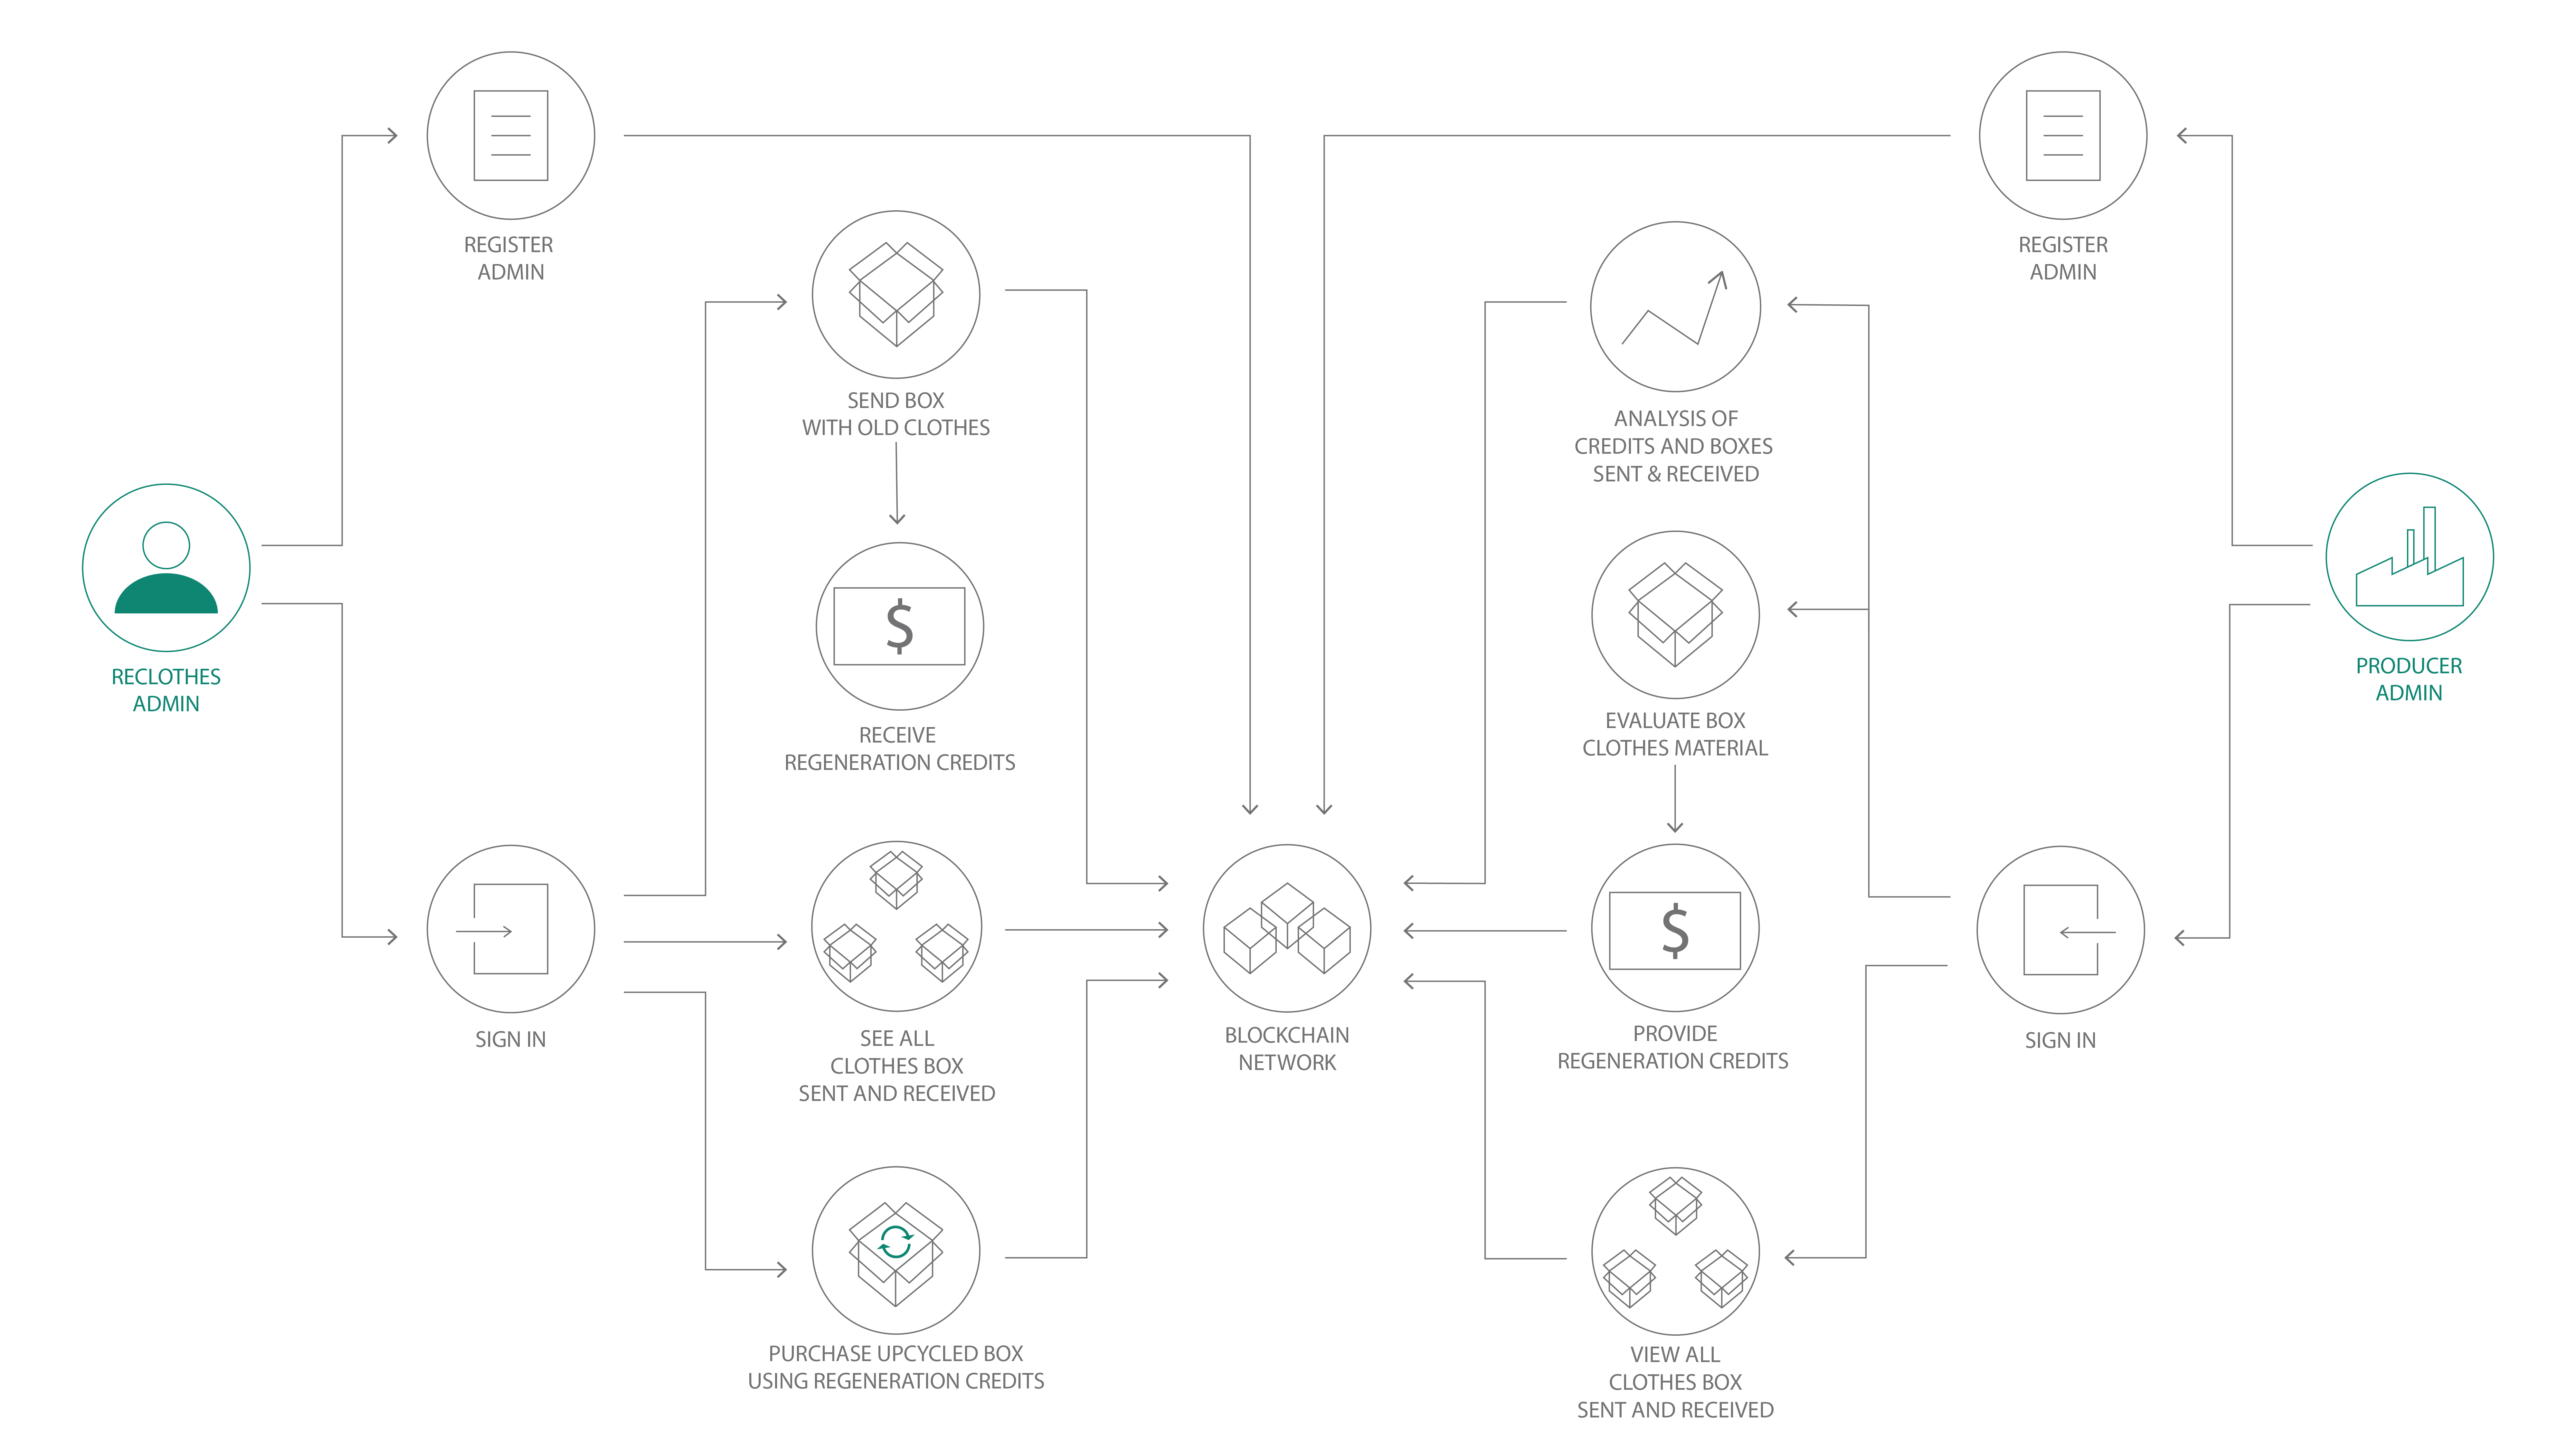
\includegraphics[totalheight=10cm]{img/use_case2.png}
	\caption{UseCase 2}
	\label{fig:usecase2}
\end{figure}


\section{Smart Contract}

All the smart contract are developed in Solidity. 

Both the Fabric contracts are use the \texttt{fabric-chaincode-evm} in order to allow Solidity code into fabric network

\begin{outline}[enumerate]
    \1 \textbf{Hyperledger Fabric}
    \2 \textbf{User Contract}: handle the the User side, registration and interactions phase.
    \2 \textbf{Producer Contract}: handle the interaction from Reclothes to Producers.
    
    \1 \textbf{Ethereum}
    \2 \textbf{ERC20 Contract}: it's a standard smart contract with a Max Supply fixed to 100.000.000 .
    The Contract run over Ropsten network and we access to it through the Infura node.
\end{outline}

\subsection{User Contract} 

\paragraph{Data Structure}
The model of the data structures is divided inside 4 structs:

\begin{outline}[enumerate]
    \1 \textbf{User}: model all users data
    \1 \textbf{Admin}: model Reclothes Admin data
    \1 \textbf{PointsTransaction}: Model transactions data and incorporate \texttt{TransactionType} used to identify the flows
    \1 \textbf{ClothesBox}: The box sent with old clothes 
\end{outline}

\begin{lstlisting}[language=Solidity]
        // model a user
        struct User {
            address userAddress;    // User address (inside fabric environment)
            address publicAddress;  // external eth public address of User Admin
            string firstName;
            string lastName;
            string email;
            uint points;            // Fabric points amount
            bool isRegistered;      // Flag for internal use
            uint numTransaction;    // number of transactions performed
            mapping(uint => PointsTransaction) userTransactions;
            uint numBox;            // number of box transaction evaluated
            mapping(uint => ClothesBox) box;
        }
    
        // model a admin
        struct Admin {
            address adminAddress;   // Admin address (inside fabric environment)
            address publicAddress;  // external eth public address of Admin
            string name;
            bool isRegistered;      // Flag for internal use
        }
    
        // model points transaction
        enum TransactionType { Earned, Redeemed }
        struct PointsTransaction {
            uint points;
            TransactionType transactionType;
            address userAddress;    // user address involved
            address adminAddress;   // admin address involved
        }
    
        // model clothes box to ship
        struct ClothesBox {
            address userAddress; // reclothes-producer Admin
            uint tshirt;        // Number of item
            uint pants;         // Number of item
            uint jacket;        // Number of item
            uint other;         // Number of item
            bool isEvaluated;   // Flag to check if box evaluation is performed
            uint points;        // fabric value amount of the box
        }
\end{lstlisting}

\paragraph{Transactions}

There's two functions that performs transaction from and to Reclothes:

\begin{outline}[enumerate]
    \1 \textbf{earnPoints}: It's an internal function called by \texttt{sendBox} function. 
    It performs the fabric points transaction from Reclothes to User.
    \1 \textbf{usePoints}: performs the fabric points transaction when the User purchase item by 
    Reclothes store.
\end{outline}

\begin{lstlisting}[language=Solidity]
    //update users with points earned
    function earnPoints (uint _points, address _userAddress ) onlyAdmin(msg.sender) internal {

      // verify user address
      require(users[_userAddress].isRegistered, "User address not found");

      // update user account
      users[_userAddress].points = users[_userAddress].points + _points;

      PointsTransaction memory earnTx = PointsTransaction({
        points: _points,
        transactionType: TransactionType.Earned,
        userAddress: _userAddress,
        adminAddress: admins[msg.sender].adminAddress
      });

      // add transction
      transactionsInfo.push(earnTx);

      users[_userAddress].userTransactions[users[_userAddress].numTransaction] = earnTx;
      users[_userAddress].numTransaction++;

      usersTransactions[totTx] = earnTx;
      totTx++;

    }


    //Update users with points used
    function usePoints (uint _points) onlyUser(msg.sender) public {

      // verify enough points for user
      require(users[msg.sender].points >= _points, "Insufficient points");

      // update user account
      users[msg.sender].points = users[msg.sender].points - _points;

      PointsTransaction memory spendTx = PointsTransaction({
        points: _points,
        transactionType: TransactionType.Redeemed,
        userAddress: users[msg.sender].userAddress,
        adminAddress: 0
      });

      // add transction
      transactionsInfo.push(spendTx);

      users[msg.sender].userTransactions[users[msg.sender].numTransaction] = spendTx;
      users[msg.sender].numTransaction++;

      usersTransactions[totTx] = spendTx;
      totTx++;
    }
\end{lstlisting}


\subsection{Producer Contract}

\paragraph{Data Structure}
The model of the data structures is divided inside 3 structs:

\begin{outline}[enumerate]
    \1 \textbf{Producer}: model all producers data
    \1 \textbf{Admin}: model Reclothes Admin data
    \1 \textbf{ClothesBox}: The box sent with old clothes 
\end{outline}

\begin{lstlisting}[language=Solidity]
    // model a producer
    struct Producer {
        address adminAddress;   // Producer Admin address (inside fabric environment)
        address publicAddress;  // external eth public address of Producer Admin
        string name;            // Producer admin name
        bool isRegistered;      // Flag for internal use
        uint numBox;            // number of box transactions evaluated
        uint pointsProvided;    // amount of points provided by own evaluations
        mapping(uint => ClothesBox) box;
    }

    // model a admin
    struct Admin {
        address adminAddress;   // Admin address (inside fabric environment)
        address publicAddress;  // external eth public address of Admin
        string name;            // Admin name
        bool isRegistered;      // Flag for internal use
        uint numBox;            // number of box transaction evaluated
        uint creditSpent;       // amount of points provided by own evaluations
        mapping(uint => ClothesBox) box;
    }

    struct ClothesBox {
        address adminAddress; // reclothes-producer Admin
        uint tshirt;        // Number of item
        uint pants;         // Number of item
        uint jacket;        // Number of item
        uint other;         // Number of item
        bool isEvaluated;   // Flag to check if box evaluation is performed
        uint points;        // fabric value amount of the box

        //mapping(uint => Clothes) clothes;
    }
\end{lstlisting}

\paragraph{Transactions}

There's two functions that perform transactions from and to Reclothes:

\begin{outline}[enumerate]
    \1 \textbf{evaluateBox}: function called by Producer to evaluate box materials, sent by Reclothes, 
    to send Regeneration Credits.
    \1 \textbf{buyUpcycledBox}: function called by Reclothes Admin that spend earned Regeneration Credits
    to purchase upcycled clothes by Producer. 
\end{outline}

\begin{lstlisting}[language=Solidity]
    // Evaluate Old Box
    function evaluateBox(uint _points) onlyProducer() public {
        //check correct pending request index
        require(evaluatedIndex < pendingIndex, "No more pending request");

        //check if evaluation is done
        require(!pendingBox[evaluatedIndex].isEvaluated, "Request just evaluated");

        //pop pending request
        ClothesBox storage box = pendingBox[evaluatedIndex];

        //update box transaction
        box.isEvaluated = true;
        box.points = _points;

        //add evaluated box
        evaluatedBox[evaluatedIndex] = box;
        evaluatedIndex++;

        debtPoints += _points;
        totPointsProvided += _points;
    }

    function buyUpcycledBox(uint _tshirt, uint _pants, uint _jackets, uint _other, uint _points) onlyAdmin() public {
        require(debtPoints >= _points, "Not enought credits accumulated in old material boxes");

        ClothesBox memory box = ClothesBox({
         adminAddress: msg.sender,
         tshirt: _tshirt,
         pants: _pants,
         jacket: _jackets,
         other: _other,
         isEvaluated: true,
         points: _points
        });

        admins[msg.sender].box[admins[msg.sender].numBox] = box;
        admins[msg.sender].numBox++;
        admins[msg.sender].creditSpent += _points;

        //add upcycled box
        upCycledBox[upCycledIndex] = box;
        upCycledIndex++;

        debtPoints -= _points;
        totBoxNew++;
    }

\end{lstlisting}

\subsection{ERC20 Contract}

It's a standard ERC20 token with the following features:

\begin{outline}
    \1 \textbf{Symbol}: CO2
    \1 \textbf{Name}: CarbonToken
    \1 \textbf{Total supply}: 100000000
    \1 \textbf{Decimals}: 18
\end{outline}

The main features of the contract are describer by ERC20 interface

\begin{lstlisting}[language=Solidity]
    contract ERC20Interface {
        function totalSupply() public constant returns (uint);
        function balanceOf(address tokenOwner) public constant returns (uint balance);
        function allowance(address tokenOwner, address spender) public constant returns (uint remaining);
        function transfer(address to, uint tokens) public returns (bool success);
        function approve(address spender, uint tokens) public returns (bool success);
        function transferFrom(address from, address to, uint tokens) public returns (bool success);
    
        event Transfer(address indexed from, address indexed to, uint tokens);
        event Approval(address indexed tokenOwner, address indexed spender, uint tokens);
    }
\end{lstlisting}

\section{Network Architecture}

The network Architecture build for the application includes:

\begin{outline}[enumerate]
    \1 \textbf{1 Orderer} organization with \textit{1 ordered} running

    \1 \textbf{3 Organizations} each with 1 peer, Peer0, running
    \2 \textit{Org1}: User Organization
    \2 \textit{Org2}: Reclothes Admin Organization 
    \2 \textit{Org3}: Producer Organization

    \1 \textbf{2 Channels}
    \2 \textit{Chanel12}: It's the cannel between Org1 and Org2 and allow the comunication between User and Reclothes
    \2 \textit{Chanel23}: It's the cannel between Org2 and Org3 and allow the comunication between Reclothes and Producer
\end{outline}

\begin{figure}[h!]
	\centering
	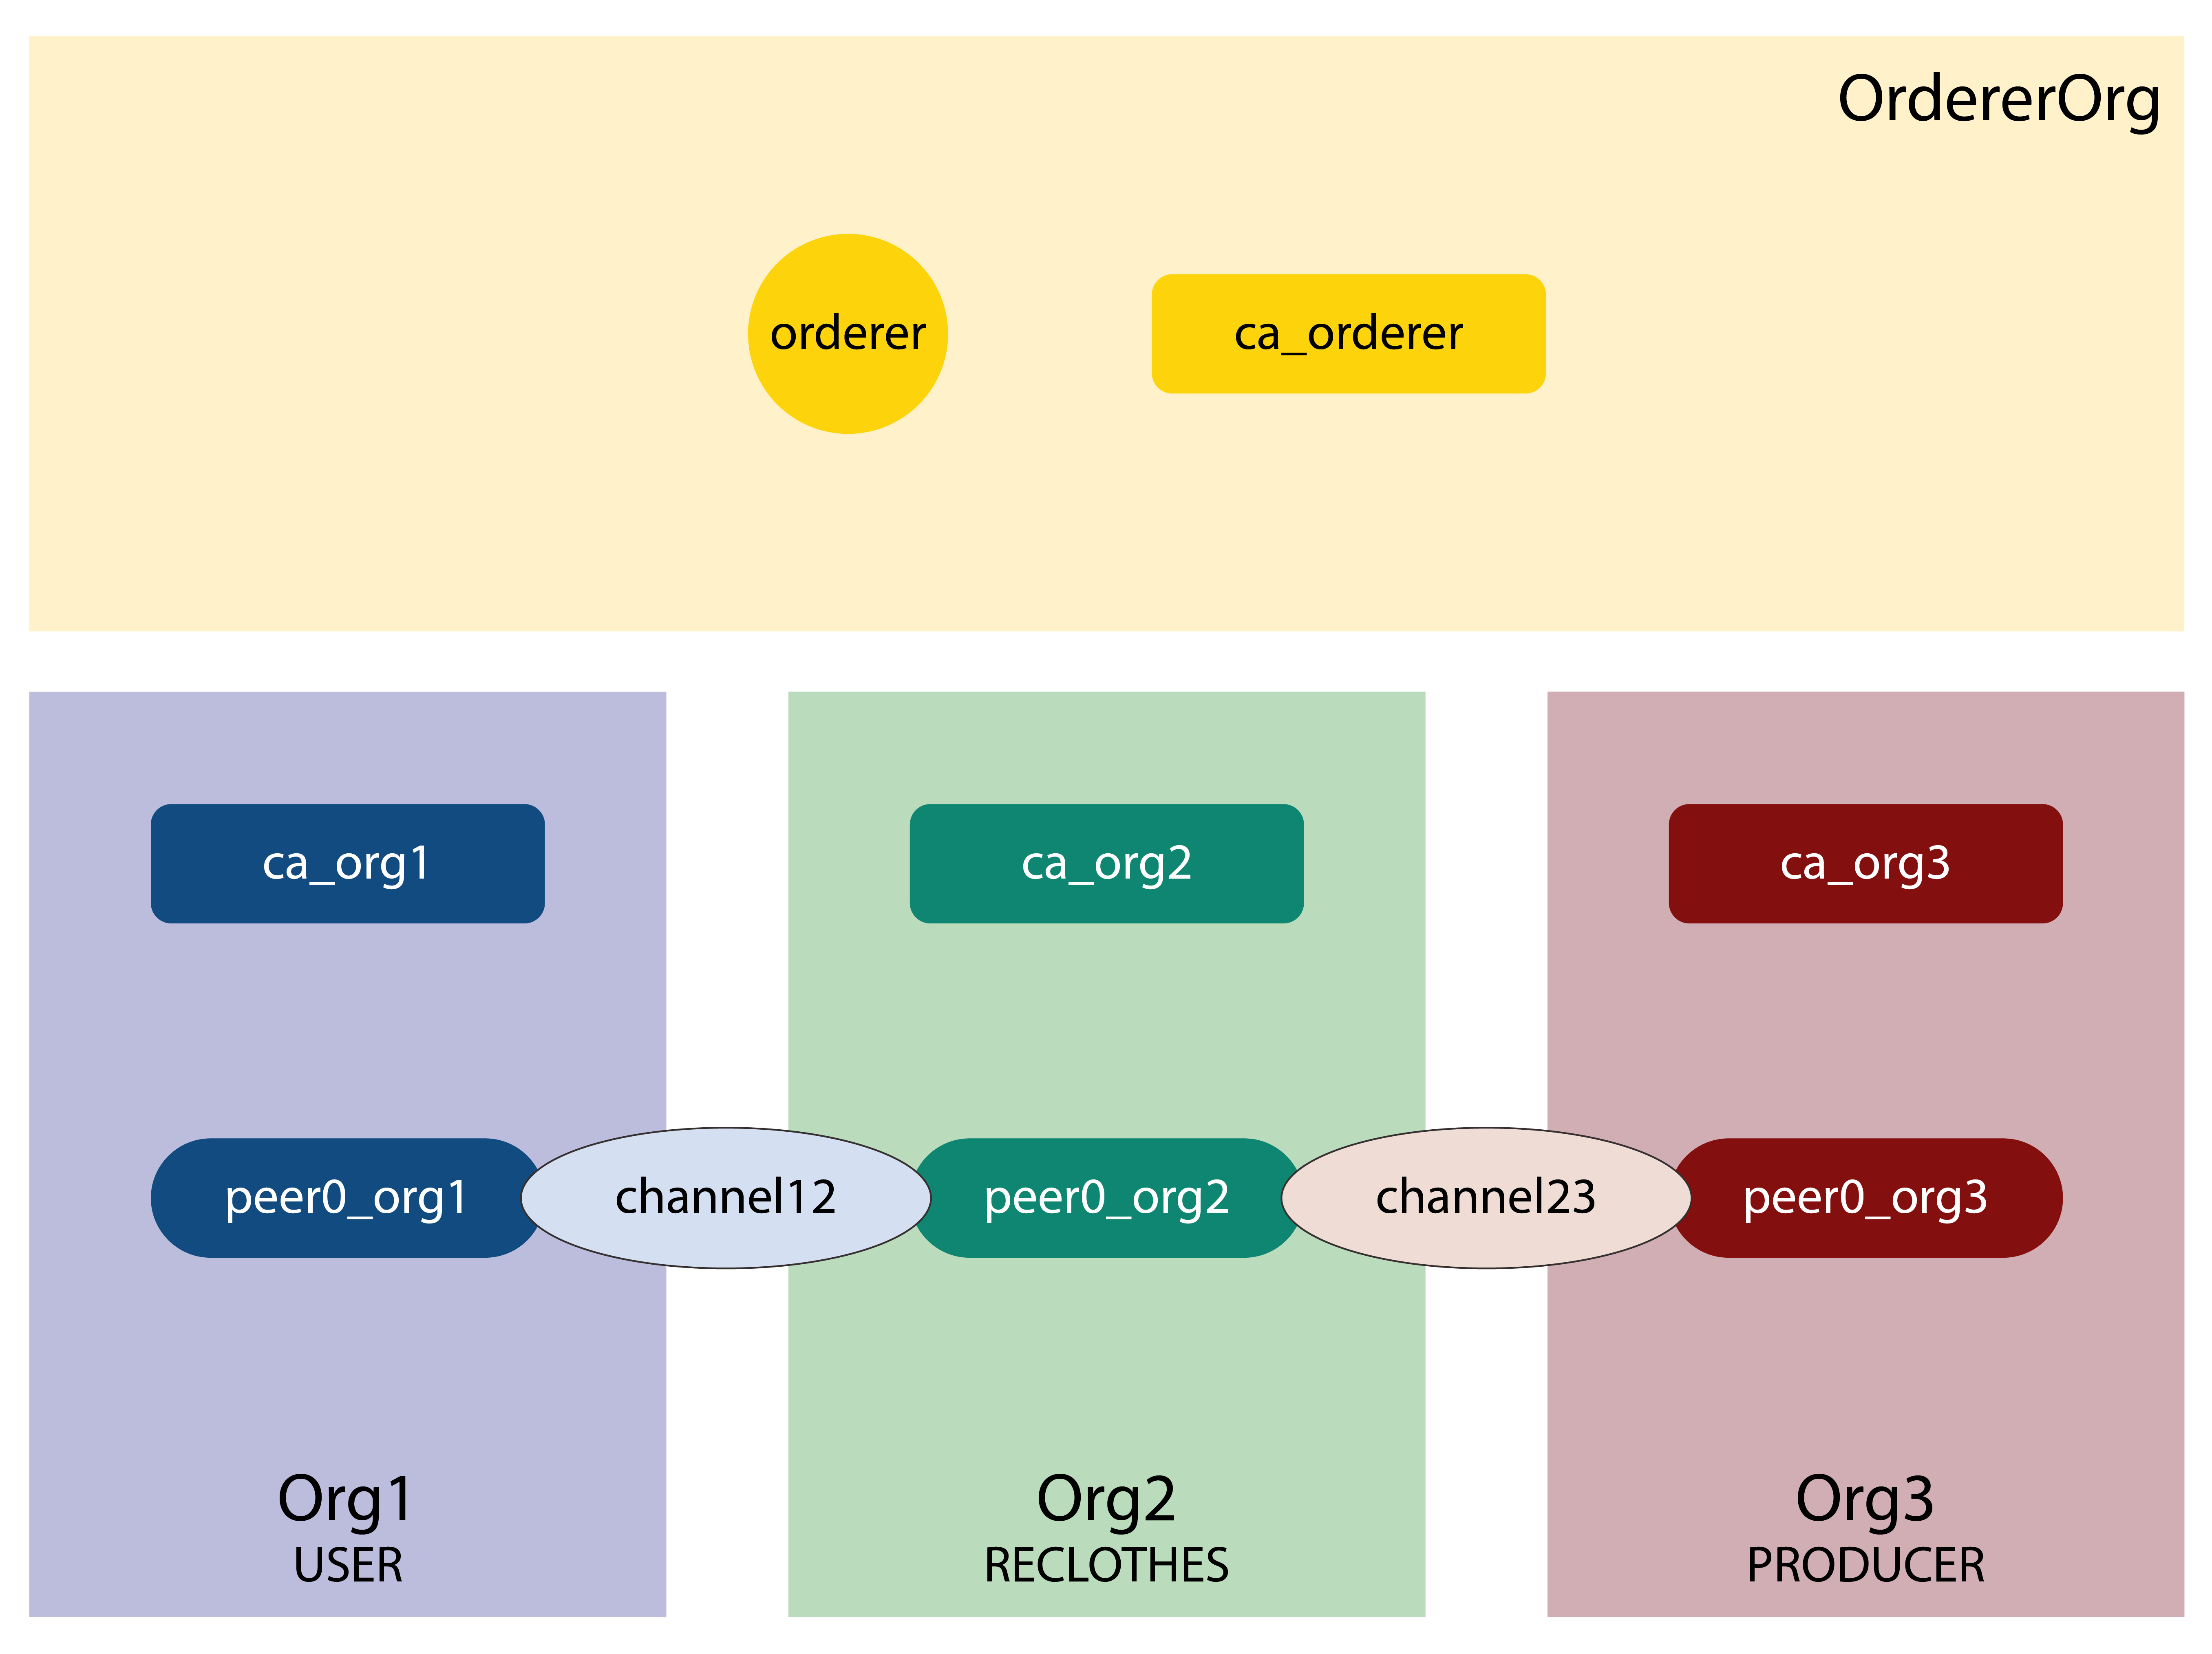
\includegraphics[totalheight=8cm]{img/fabric_network.png}
	\caption{Fabric Network}
	\label{fig:fabric_network}
\end{figure}

\subsection{Fabric Network}

The Figure show how components interact each other. We could separate components into 2 categories,
inside and outside Fabric Network. First of all we need to describe the components involved :

\begin{outline}
    \1 \textbf{Web3 App}: It's the Dapp and the Client connection to the network
    \1 \textbf{Channel}: It's the channel above which transfert data 
    \1 \textbf{CA}: It's the Certification Authority in charge of release certificates.
    \1 \textbf{Peer}: It's "Fabric node", the endpoint of the internal network. It own by specific CA with 
    fixed permissions, linked to the connected channels. 
    \1 \textbf{evm SC}: It's the Ethereum Virtual Machine Chaicode, used to run Solidity Smart Contract. The chaincode 
    is installed over the peer.
    \1 \textbf{ledger}: It's the ledger associated to the channel connected. There's a 1 to 1 association 
    between ledger and channel.
    \1 \textbf{CC}: It's the \textit{Consortium}, It's associated to the channel, manage ownerships and 
    It include a set of Organizations allowed. 
    \1 \textbf{Docker}: The network components run inside docker containers. 
\end{outline}

\begin{figure}[h!]
	\centering
	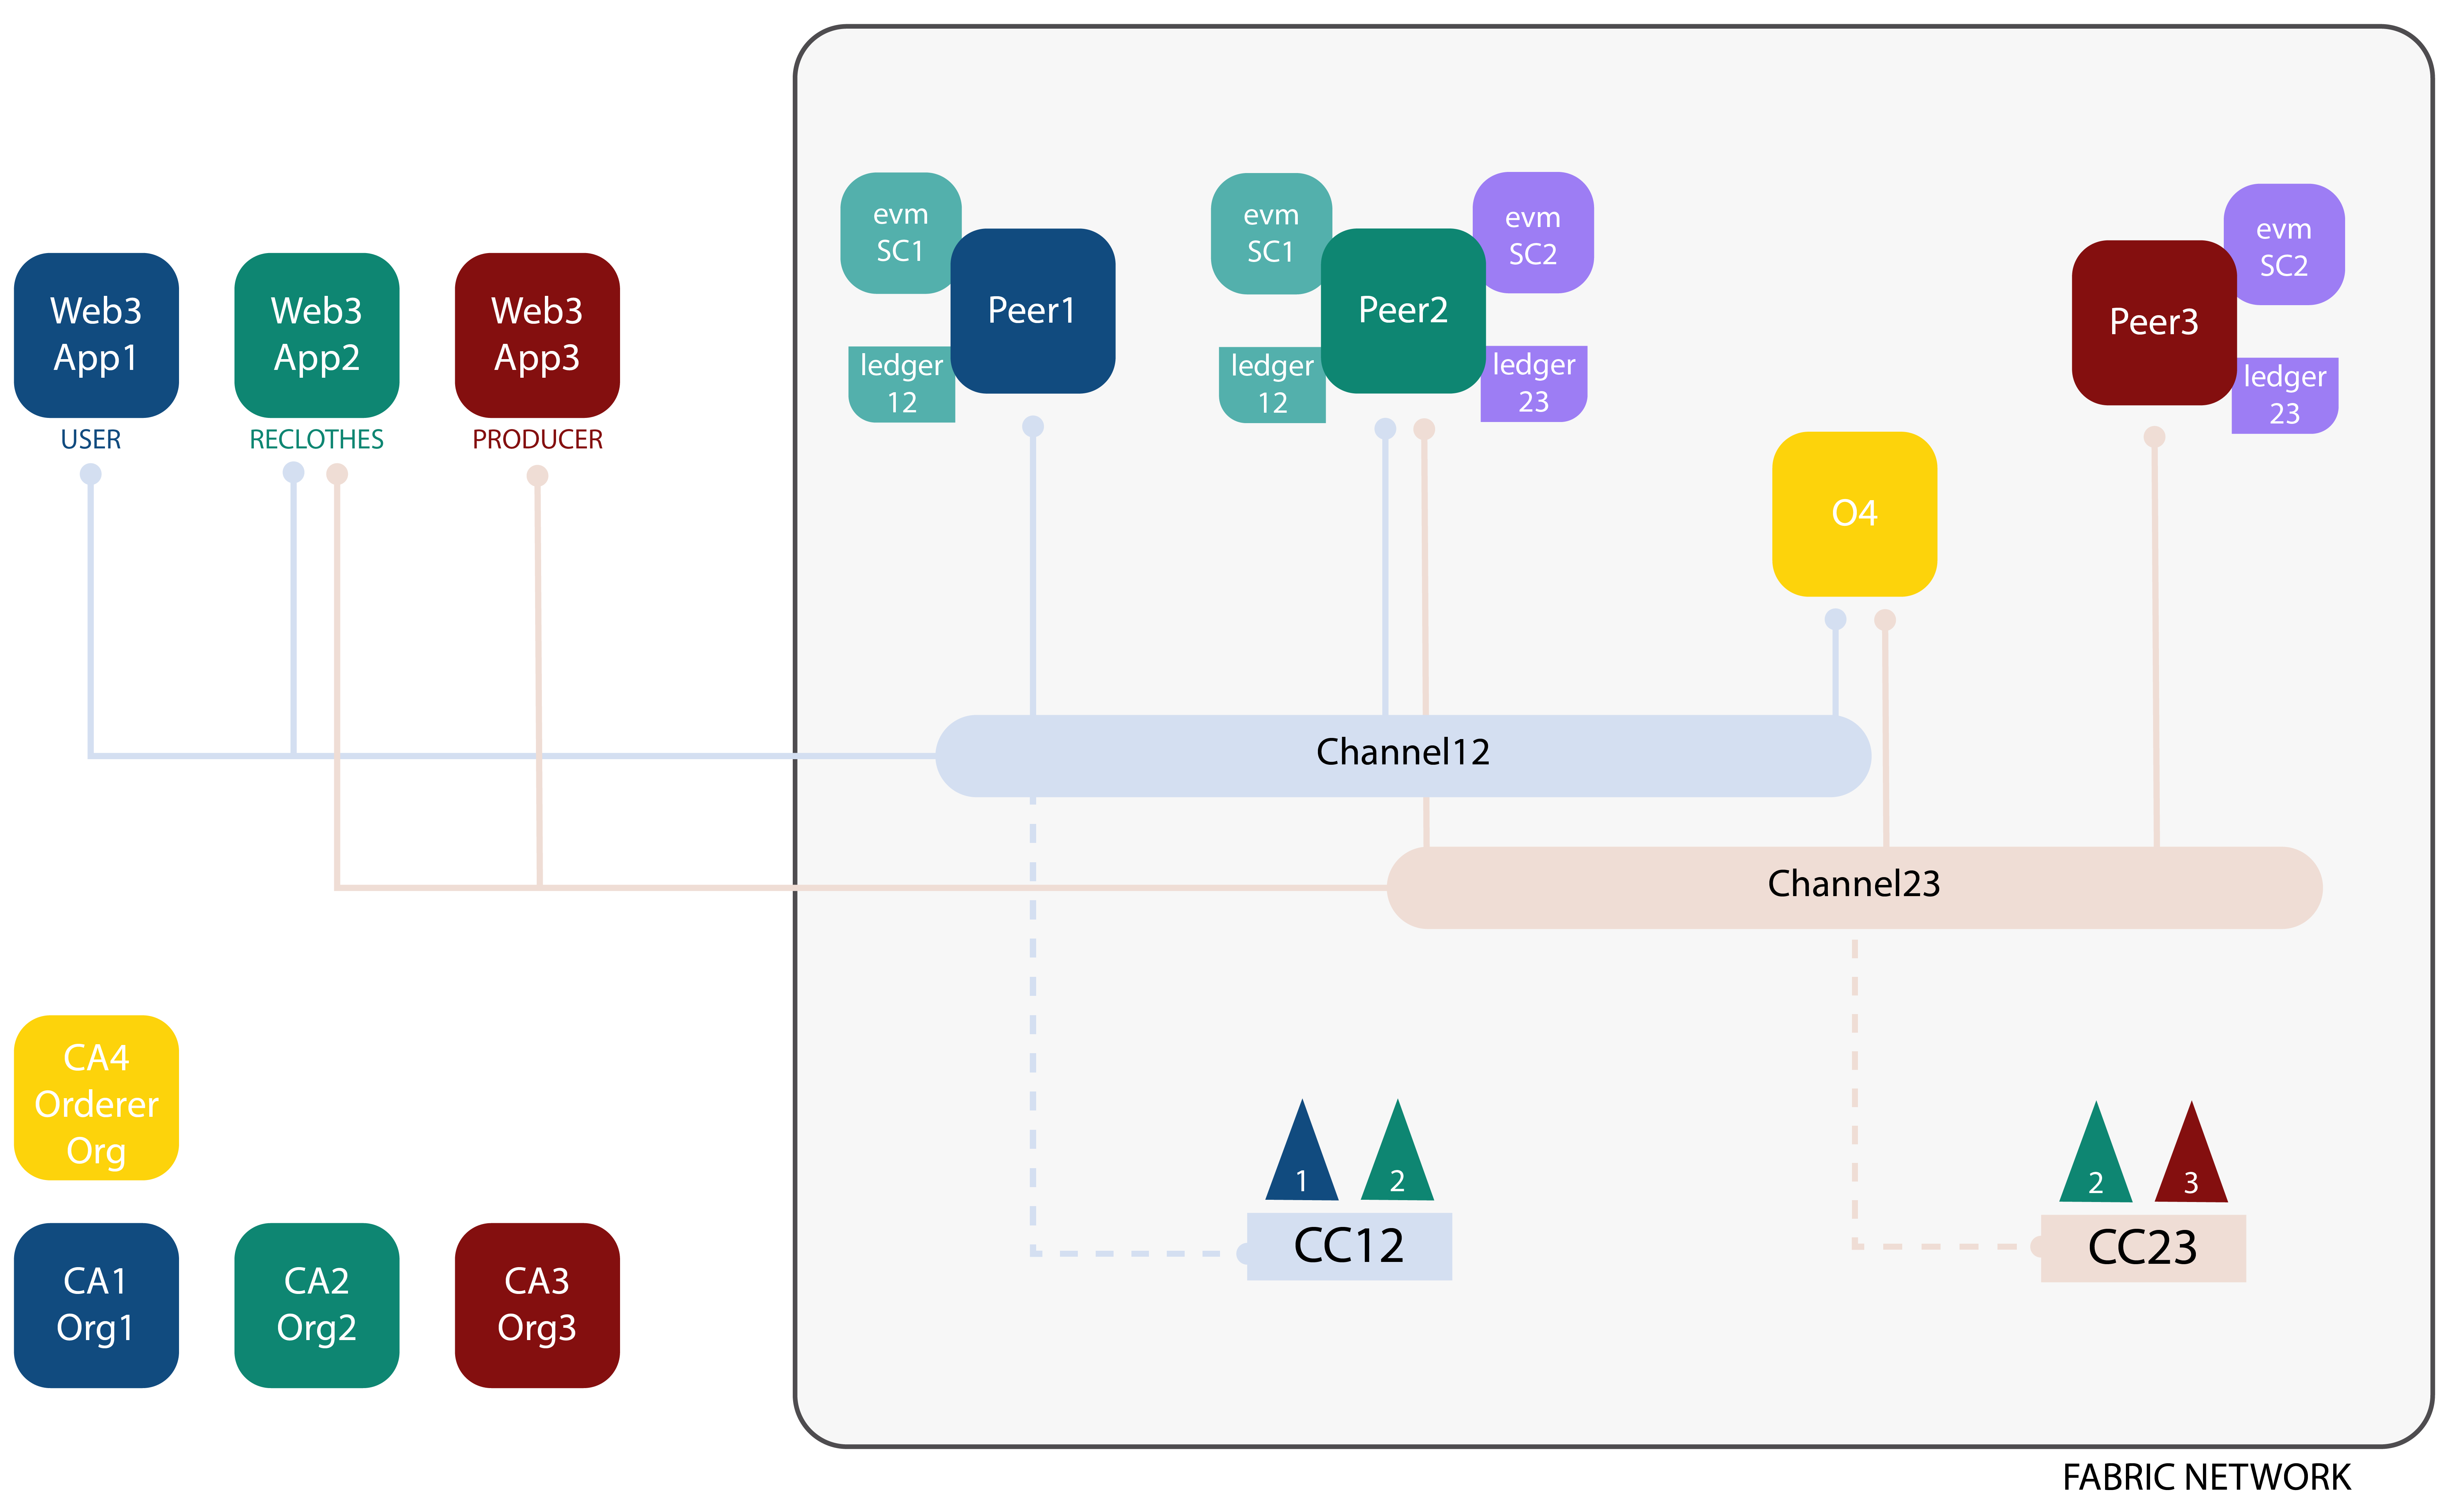
\includegraphics[totalheight=10cm]{img/network.png}
	\caption{Fabric Network Components}
	\label{fig:network}
\end{figure}

The \textit{chaincode} it's invoked calling the evm chaincode by the \textit{App} Client, using the channel communication.
Than the chaincode installed over the peer once is invoked agreed to the request and invoke the chaincode("smart contract")
method. Once the method returns, the chaincode forward the reply to the App client. The Dapp forward the
answer to the \textit{Orderer} peer that validate the response, create a new block, add it to the chain,
communicate it to the peer in order to syncronize the network and updating the Ledger World State.

\subsubsection{Config File}

To design and set up network components and rules, It's wrote the \texttt{config.yaml} file.
The network is structured in the following lines of code:

\begin{lstlisting}
    Organizations:
    - &OrdererOrg
        Name: OrdererOrg
        ID: OrdererMSP
        MSPDir: crypto-config/ordererOrganizations/example.com/msp
        Policies:
            Readers:
                Type: Signature
                Rule: "OR('OrdererMSP.member')"
            Writers:
                Type: Signature
                Rule: "OR('OrdererMSP.member')"
            Admins:
                Type: Signature
                Rule: "OR('OrdererMSP.admin')"

    - &Org1
        Name: Org1MSP
        ID: Org1MSP
        MSPDir: crypto-config/peerOrganizations/org1.example.com/msp
        Policies:
            Readers:
                Type: Signature
                Rule: "OR('Org1MSP.admin', 'Org1MSP.peer', 'Org1MSP.client')"
            Writers:
                Type: Signature
                Rule: "OR('Org1MSP.admin', 'Org1MSP.client')"
            Admins:
                Type: Signature
                Rule: "OR('Org1MSP.admin')"
        AnchorPeers:
            - Host: peer0.org1.example.com
              Port: 7051

    - &Org2
        Name: Org2MSP
        ID: Org2MSP
        MSPDir: crypto-config/peerOrganizations/org2.example.com/msp
        Policies:
            Readers:
                Type: Signature
                Rule: "OR('Org2MSP.admin', 'Org2MSP.peer', 'Org2MSP.client')"
            Writers:
                Type: Signature
                Rule: "OR('Org2MSP.admin', 'Org2MSP.client')"
            Admins:
                Type: Signature
                Rule: "OR('Org2MSP.admin')"
        AnchorPeers:
            - Host: peer0.org2.example.com
              Port: 8051

    - &Org3
        Name: Org3MSP
        ID: Org3MSP
        MSPDir: crypto-config/peerOrganizations/org3.example.com/msp
        Policies:
            Readers:
                Type: Signature
                Rule: "OR('Org3MSP.admin', 'Org3MSP.peer', 'Org3MSP.client')"
            Writers:
                Type: Signature
                Rule: "OR('Org3MSP.admin', 'Org3MSP.client')"
            Admins:
                Type: Signature
                Rule: "OR('Org3MSP.admin')"
        AnchorPeers:
            - Host: peer0.org3.example.com
              Port: 9051


                                        ...
                                        ...
                                        ...

Profiles:

    OrdererGenesis:
        <<: *ChannelDefaults
        Orderer:
            <<: *OrdererDefaults
            Organizations:
                - *OrdererOrg
            Capabilities:
                <<: *OrdererCapabilities
        Consortiums:
            SampleConsortium:
                Organizations:
                    - *Org1
                    - *Org2
                    - *Org3

    Channel12:
        Consortium: SampleConsortium
        <<: *ChannelDefaults
        Application:
            <<: *ApplicationDefaults
            Organizations:
                - *Org1
                - *Org2
            Capabilities:
                <<: *ApplicationCapabilities
    Channel23:
        Consortium: SampleConsortium
        <<: *ChannelDefaults
        Application:
            <<: *ApplicationDefaults
            Organizations:
                - *Org2
                - *Org3
            Capabilities:
                <<: *ApplicationCapabilities    
\end{lstlisting}

    \subsubsection{End to End Interactions} 
    Going deeper, the Figure show the flow of the end to end communication. How all the components are boxed 
    inside the Peer component. The Fab3 map the web3 request and forward it to fabric peer. the request 
    arrive to the evmcc that invoke Solidity smart contract methods.

    \begin{figure}[h!]
        \centering
        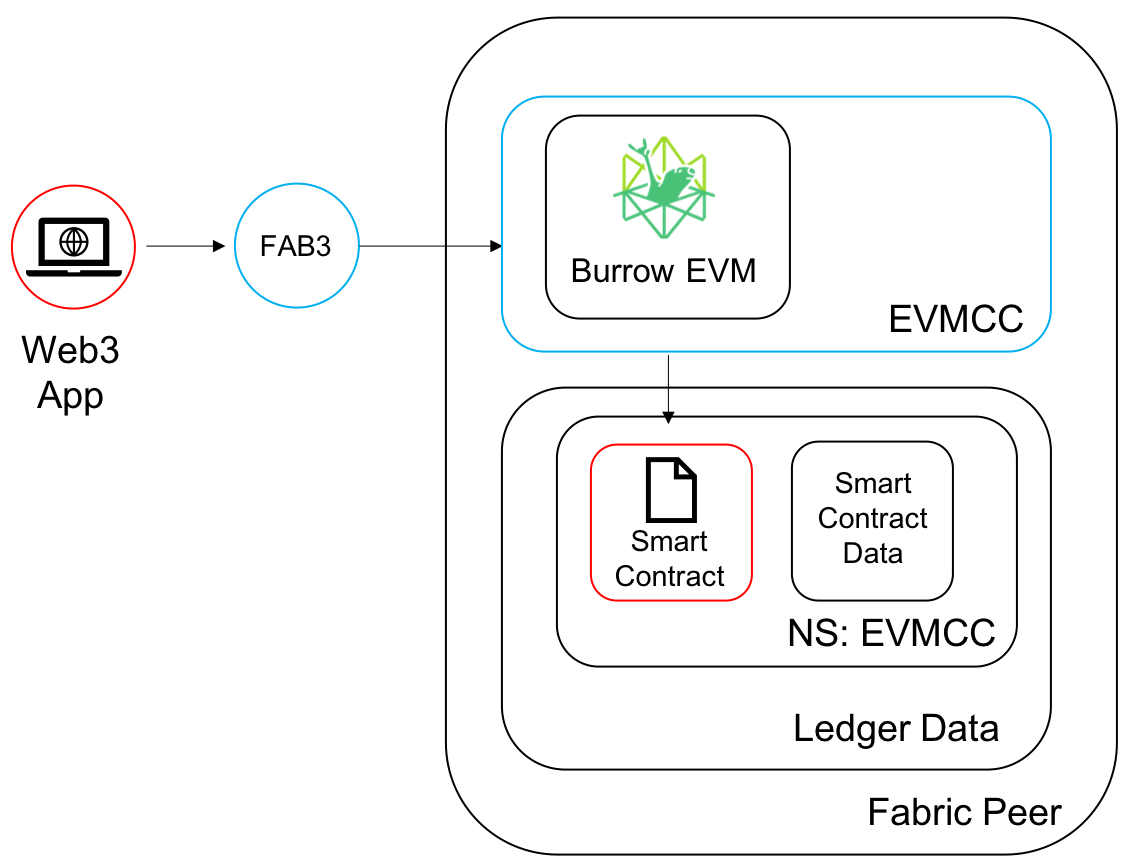
\includegraphics[totalheight=7.5cm]{img/EndToEnd.png}
        \caption{End To End}
        \label{fig:end_to_end}
    \end{figure}

    \subsubsection{Chaincode Invocations}
    The Figure below describe the internal workflow of the chaincode invocation, where's involved the 
    \textit{Client} the \textit{Peer} and the \textit{Orderer}. All the information are transfer over the 
    setted channel and in our study case, the client doesn't interact directly, but using \textit{Fab3 Proxy}
    as intermediary.

    \begin{figure}[h!]
        \centering
        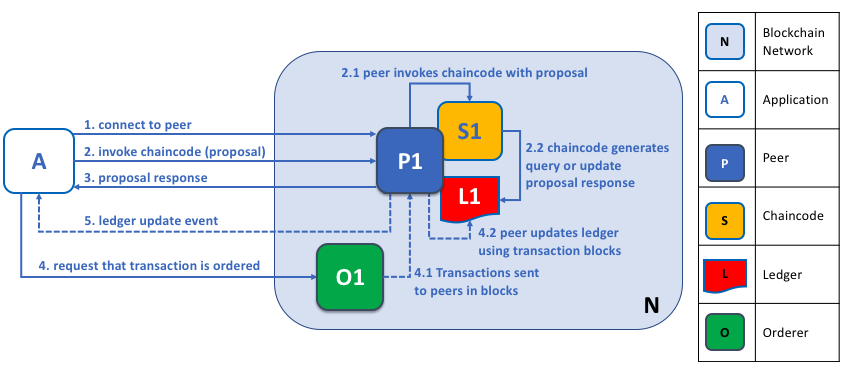
\includegraphics[totalheight=6cm]{img/sc_invokation.png}
        \caption{Smart Contract Invocation Process}
        \label{fig:sc_invokation}
    \end{figure}

\subsection{Ethereum Network - Ropsten}

To run the ERC20 token it's used the testnet Ropstan against the mainnet. 
To set up and upload own ERC20 Token over the ethereum network it's used:

\begin{outline}
    \1 \textbf{My Ether Wallet}: To upload ERC20 contract 
    \1 \textbf{Etherscan.io}: To monitor and analyze transactions over the network
    \1 \textbf{Metamask}: To create user wallets
    \1 \textbf{Infura}: To set up a node in order to use it as endpoint and communicate with the Ropsten network,
    it is used as \textit{Provider} in \textit{Web3} library.  
\end{outline}

\section{Dapp - Client}

\subsection{Thecnologies used}

To develop the client application is used the following Technologies:

\begin{outline}
    \1 \textbf{Expressjs}: It's a node.js framework that allow to develop api for own application
    \1 \textbf{Bootstrap}: To build a user friendly front-end in order to interact in the best way
    \1 \textbf{Web3}: Ethereum Javascript API, It's is a collection of libraries that allow you to interact with a local or remote ethereum node 
    \2 \textbf{web3 0.20.2}: used for dapp developments, fabric side, It's a stable version and it's the version
    used in \texttt{fabric-chaincode-evm} development
    \2 \textbf{web3 1.0.0}: used for ethereum transactions, It's a version with more functionalities but less stable.
\end{outline}

Starting from the Homepage the User is allowed to register itself as \textbf{User}, \textbf{Reclothes Admin}
or \textbf{Producer}.

\subsection{Core part of the web-app}

The technical files and flow that dapp follow to run up it's the following one.

\begin{outline}[enumerate]
    \1 \textbf{Contract Address Generation}:
    \2 This step is in charge to run a script that deploy the contract adresses to be reffered during the 
    app running.
    \3 \textbf{UserContract.js}: running the script using node command, it return the address of the deployed contract
    \3 \textbf{ProducerContract.js}: running the script using node command, it return the address of the deployed contract
    \1  \textbf{dapp.js}: there's the core file that handle the contracts invokations, set up the contract address
    referance, and connect to a specific Fab3 instance.
    \1 \textbf{app.js}: It set up the API called by the web-app, map the request and forward to \texttt{dapp.js}.
\end{outline}

\subsection{Views}

\subsubsection{Homepage}

The homepage allow user to view the feature of each User type and to access to the registration page.

\begin{figure}[h!]
    \centering
    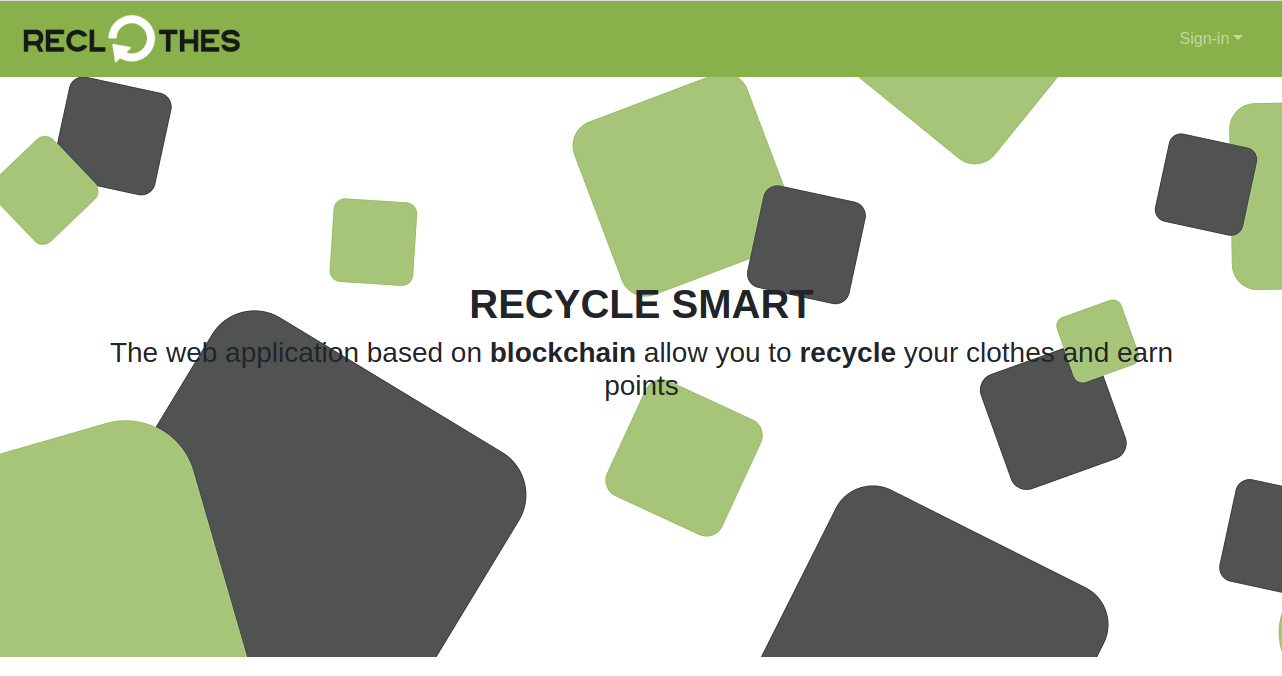
\includegraphics[totalheight=7.5cm]{img/dapp/home1.png}
    \caption{Home}
    \label{fig:home}
\end{figure}

\begin{figure}[h!]
    \centering
    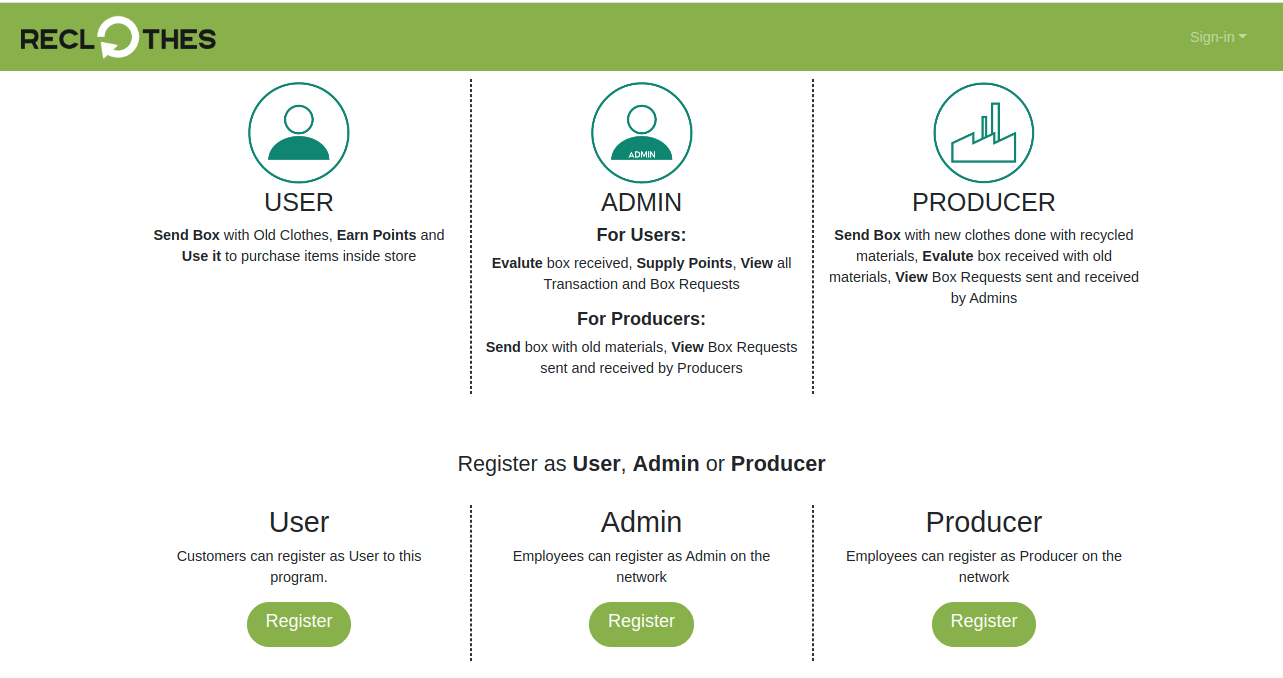
\includegraphics[totalheight=7.5cm]{img/dapp/home2.png}
    \caption{Registration Phase}
    \label{fig:registration}
\end{figure}

\subsubsection{User Page}

The User page allow to view an overview infos once the user is logged in. 

\begin{enumerate}[-]
    \item \textbf{Address}: It's the public eth address setup during registration phase. 
    \item \textbf{Points Balance}: It's the Fabric points balance earned by the user sending the boxes.
    \item \textbf{ERC20 Balance}: It's the eth balance of the public token running over eth network.
\end{enumerate}

The Figure xxxx show how to compile the form in order to send box with old clothes. It's a simulation
of the real process to sending box, that in the real case could be implemented thow a QRCode or RFID
placed over the boxes.

The Figure xxx show how should be the store, purchase items over the platform start the transaction 
process. 

There's other section about infos that user is allowed to see. \textbf{Transactions} performed over
the fabric network and \textbf{Box Requests} that's all the history about the box sent and received
with all the related informations. 

\begin{figure}[h!]
    \centering
    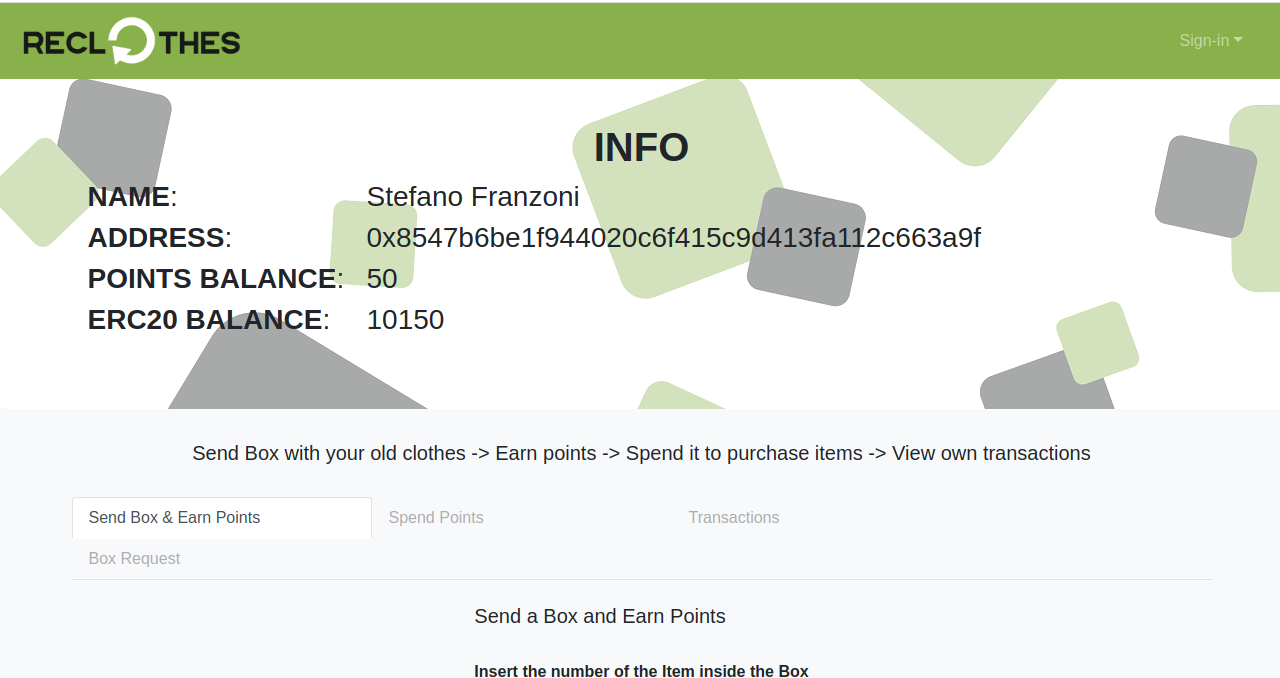
\includegraphics[totalheight=7.5cm]{img/dapp/user-info.png}
    \caption{User Info}
    \label{fig:user_info}
\end{figure}

\begin{figure}[h!]
    \centering
    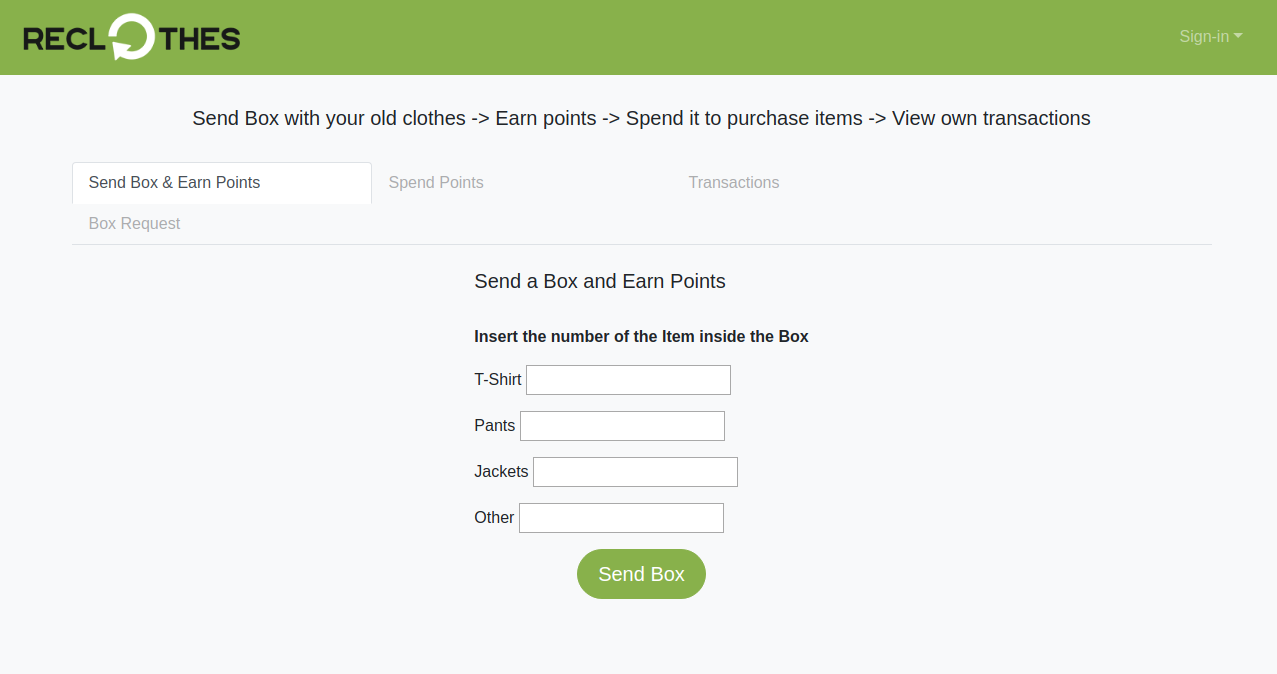
\includegraphics[totalheight=7.5cm]{img/dapp/user-send.png}
    \caption{Send Box}
    \label{fig:send_box}
\end{figure}

\begin{figure}[h!]
    \centering
    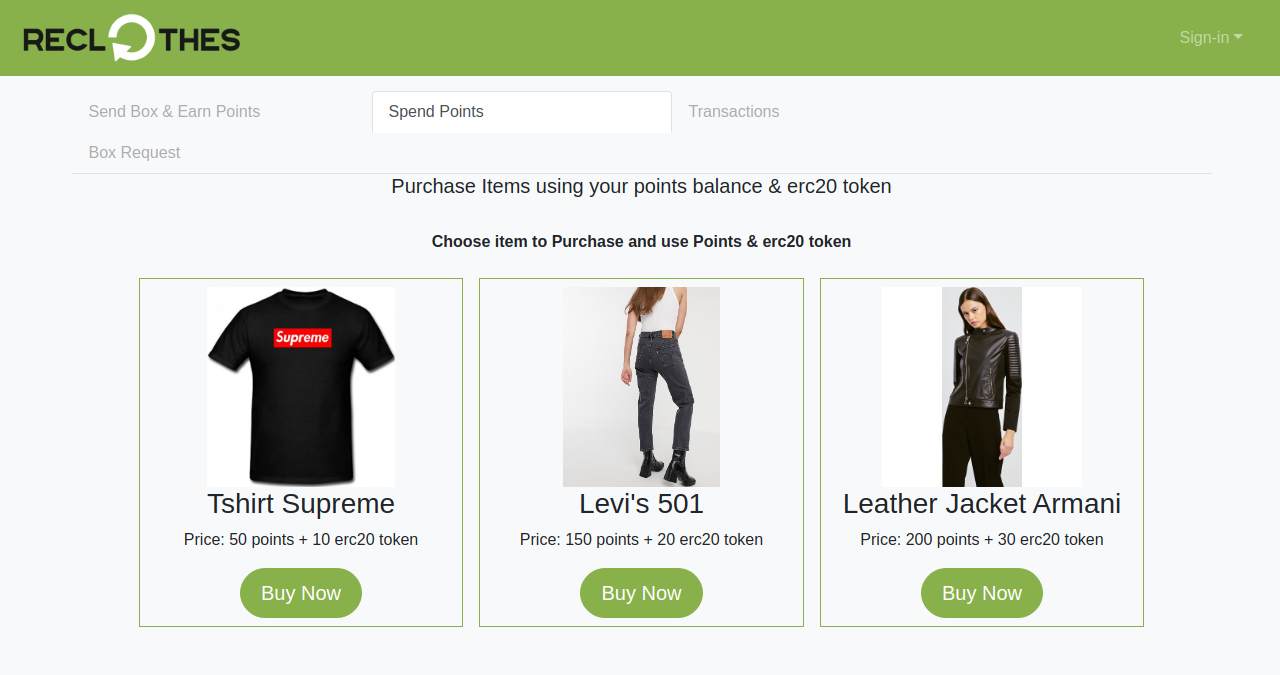
\includegraphics[totalheight=7.5cm]{img/dapp/user-buy.png}
    \caption{Purchase Clothes}
    \label{fig:purchase_clothes}
\end{figure}

\subsubsection{Reclothes Admin Page}

In the previous sections we talk about a logical split about Admin for User and Admin for Producers.
In the following views we divide the feature releated to the User type to be handled and there's a 
streight distinctions about Users and Producers.

\paragraph{Admin For Users}

This section show the view of the Admins that handle User side.

\begin{figure}[h!]
    \centering
    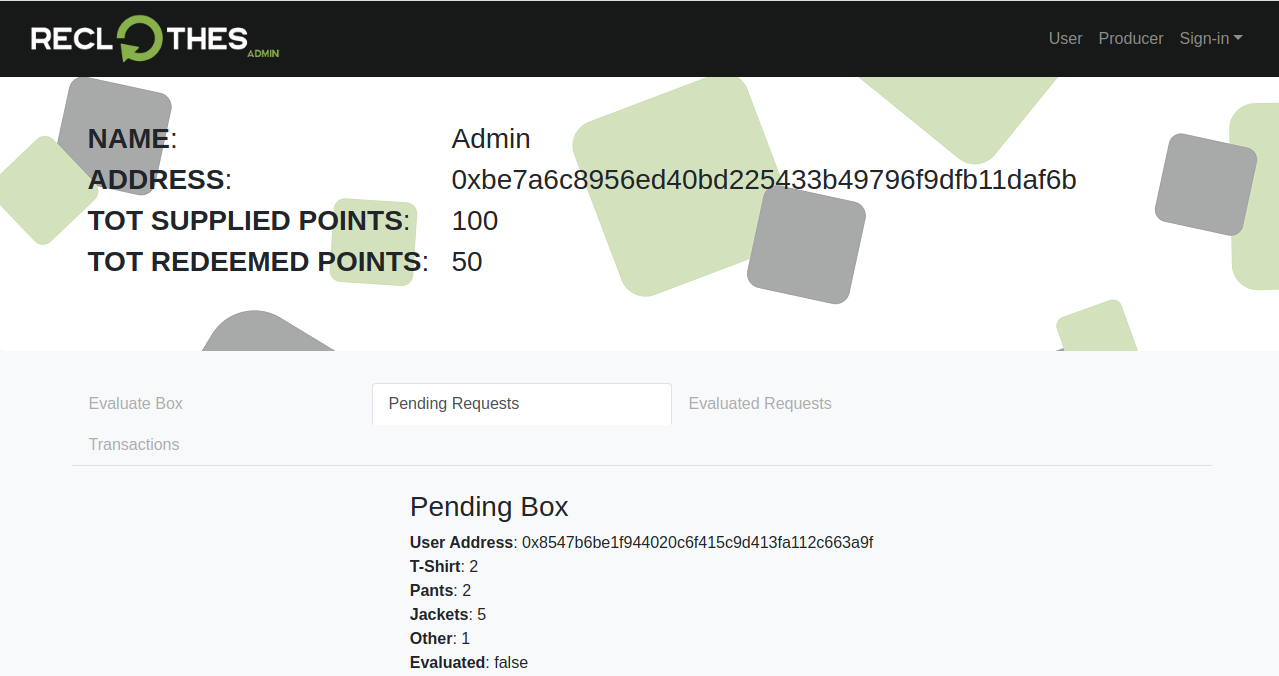
\includegraphics[totalheight=7.5cm]{img/dapp/admin-info.png}
    \caption{Admin Info}
    \label{fig:admin_info}
\end{figure}

\begin{figure}[h!]
    \centering
    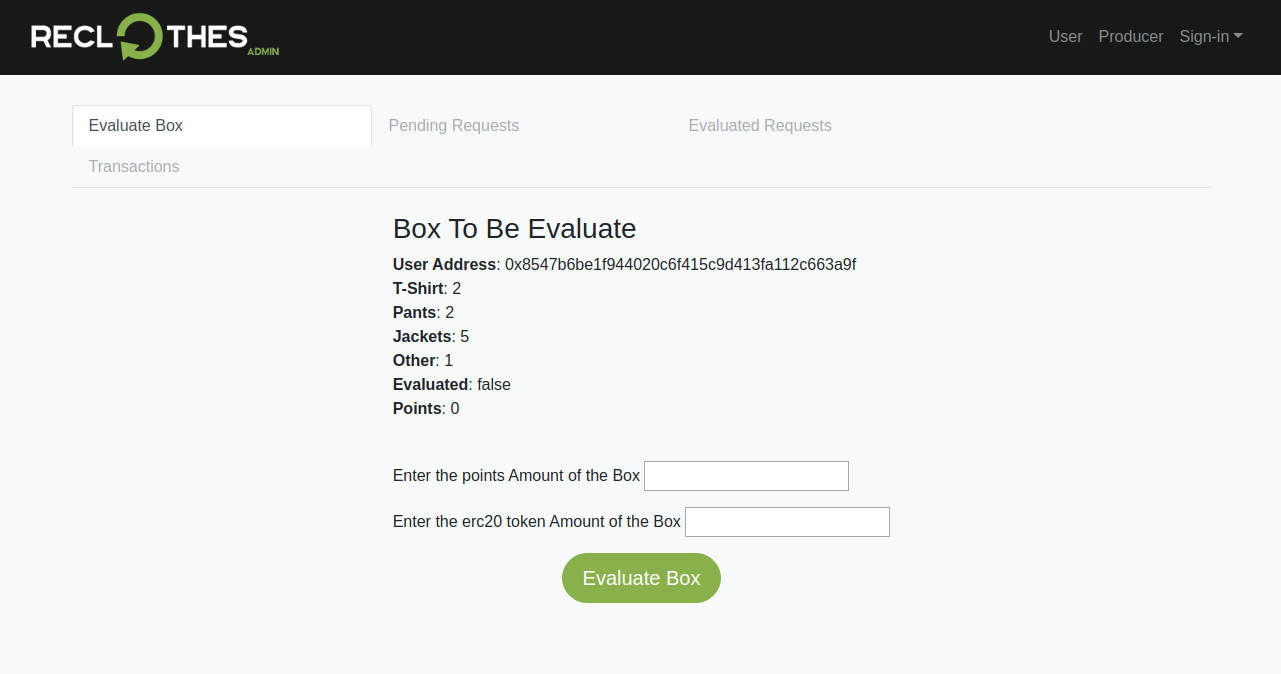
\includegraphics[totalheight=7.5cm]{img/dapp/admin-evaluate.png}
    \caption{Evaluate Box}
    \label{fig:evaluate_box}
\end{figure}

\begin{figure}[h!]
    \centering
    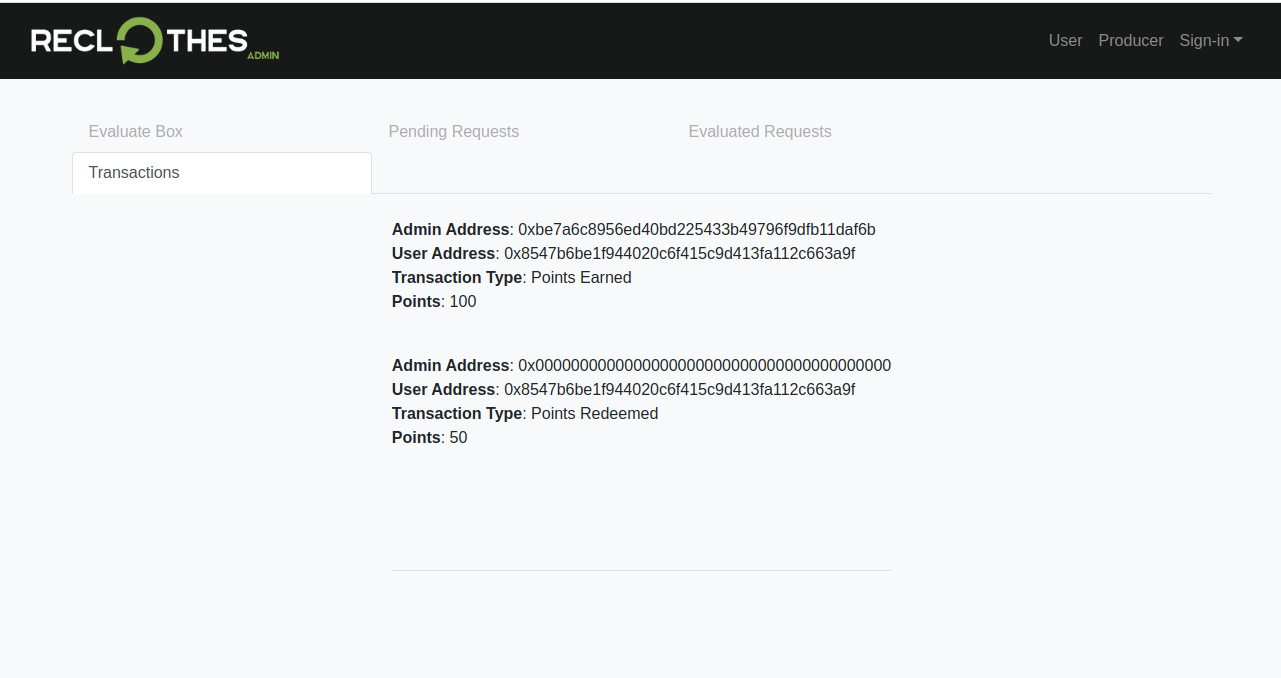
\includegraphics[totalheight=7.5cm]{img/dapp/admin-tx.png}
    \caption{Transactions}
    \label{fig:admin-tx}
\end{figure}

\paragraph{Admin For Producers}

This section show the view of the Admins that handle Producer side.

\begin{figure}[h!]
    \centering
    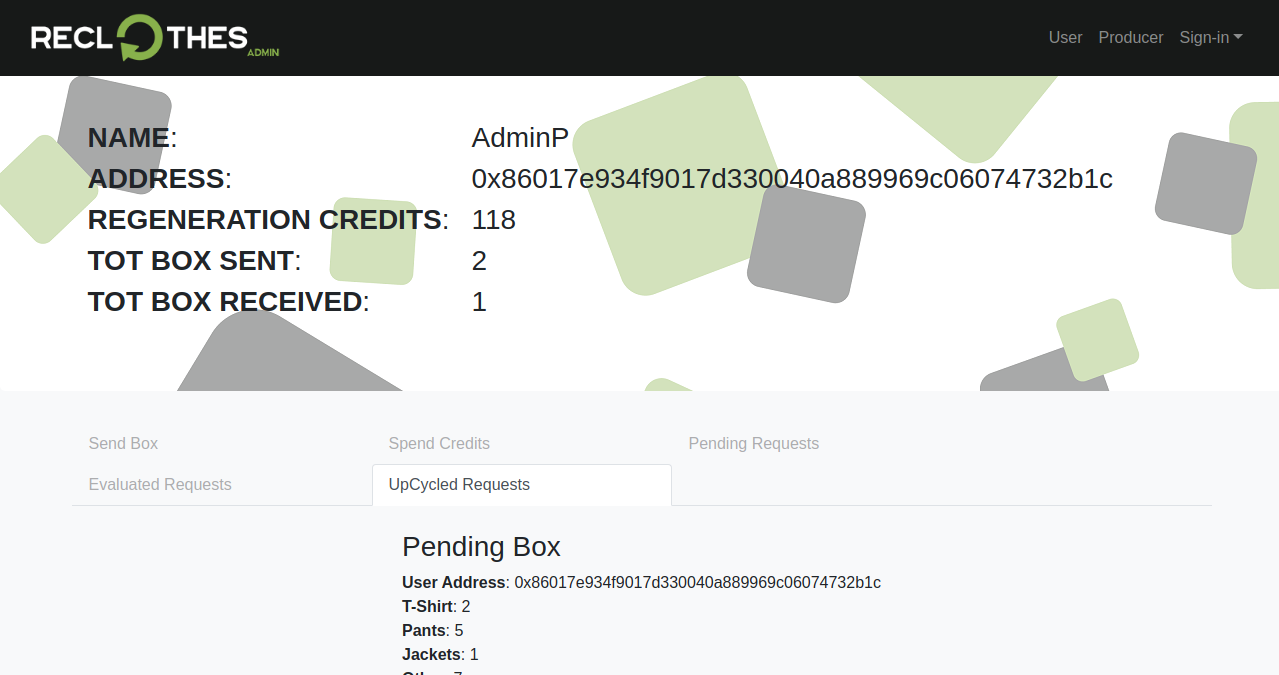
\includegraphics[totalheight=7.5cm]{img/dapp/adminp-info.png}
    \caption{Admin for Producers Info}
    \label{fig:adminp-info}
\end{figure}

\subsubsection{Producer}

This section show the view of the Producer side.

\begin{figure}[h!]
    \centering
    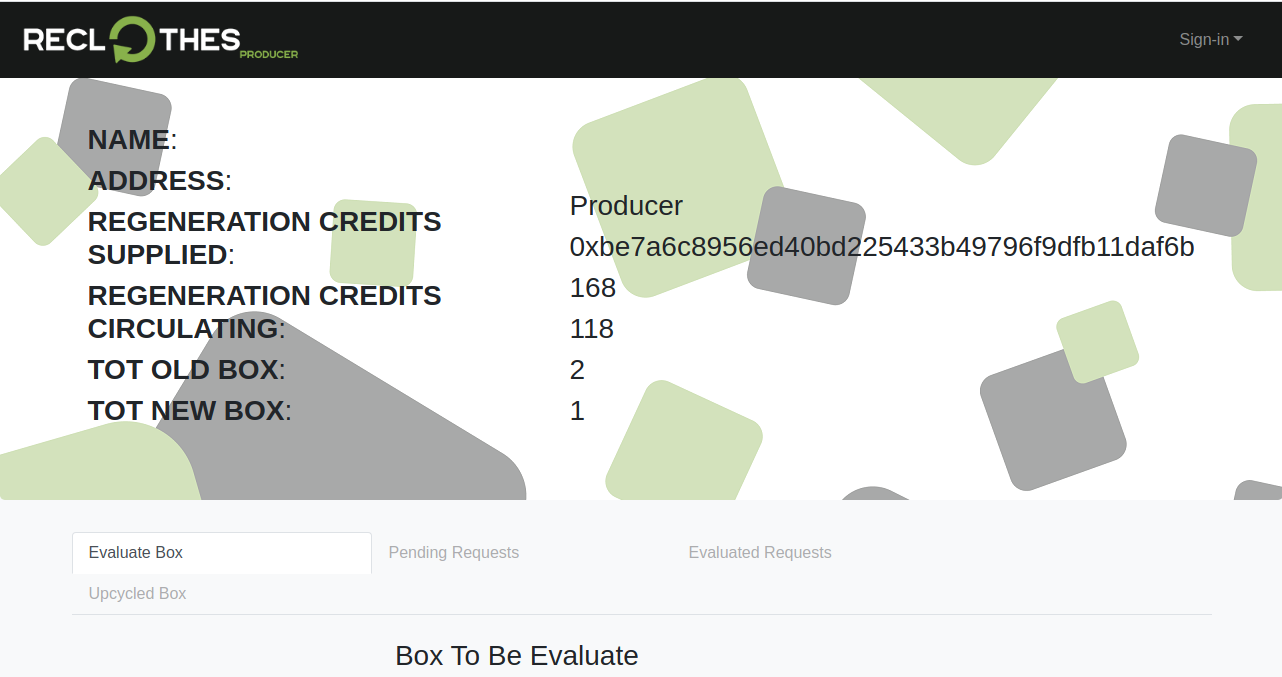
\includegraphics[totalheight=7.5cm]{img/dapp/producer-info.png}
    \caption{Producers Info}
    \label{fig:producer-info}
\end{figure}

}